\farzaneh{intro on GPU} Graphical Processing Unit (GPU) devices were originally designed for rendering graphics efficiently.
%  and outputting to a display device.
%
However, with their multi-threading capabilities providing an unprecedented computational speed, they soon went further than their original use case and got used in general purposedd computation. 
%
Nowadays, GPUs are essential in general-purpose computing particularly for applications that work with huge data and need parallelizing their heavy workloads.
%
For example, training a neural network with vast amounts of data such as audio, text or images gets boosted in speed by a GPU.
%
With GPUs being used for general purposed computing, most of the everyday users can also benefit from that.
%
For example, encryption/decryption of large data sets, and training an LLM model.
%
However, it is not always resourceful to allocate a complete GPU to a single machine when only a fraction of time or processing power it will be used.
%
Datacenter providers started to provide GPU-as-a-service(GaaS) on cloud.
%
For example: Google's Kubernetis Engine allows to share
a GPU between up to 48 tenants, while Microsoft build
GPU Paravirtualization into the Hyper-V Hypervisor, allowing VMs to share a single GPU
% also serve as a powerful platform for accelerating
% ubiquitous, non-graphical rendering tasks.
% GPUs' ability to execute thousands of threads concurrently makes them essential in general-purpose computing.
\farzaneh{importance of cloud services to deliver high throughput.}
Most of these applications involve confidential data. 
%
For example, in LLM, they work with large set of personal data based on the application, e.g., medical data.
%
In cryptography, both the plaintext and the encryption key are confidential.
%
While modern operating systems deploy
tight sandboxing and access management in order to
enforce hard boundaries between applications, recent research showed that there are several caveats in security of GPUs.
%
Research on CPUs cannot be directly applied here, mainly because the memory pattern acces and parallelism paradigm is different from CPU which introduces new attacker models including new side channel attacks.
%
% Here we look at two main category of attacks.
%
% However, its memory layout and the cost properties introduce vulnerabilities, e.g., shared memory bank conflicts.
%
\farzaneh{prior work on GPU}
%
Prior work showed several such vulenrabilities, ranging from leaking via a timing channel rooted from the unique memory access pattern of GPUs across multiple threads to shared memory (?) and register spills rooted from scheduling of multiple shaders (applications?) on a single GPU.
%
However, studying it from a language-based security is missing.
%
We propose a language-based security approach toward GPU security, that allows for undersanding the foundation of such attacks, and provide solutions that are not ad-hoc.
%
It allows for understanding the fundamentals of security in this new concurrency paradigm.
%
It provides provable security.
%
With this fundamental understanding it will also be more feasible to incorporate it with prior work on CPU, etc.
%



This is the goal of this work: the first language-based security analysis for GPU concurrency paradigm.
%
We consider two main attacks.
%
They both raised by the unique memory layout of GPU.
%
So we first briefly describe the memory layout and our attacker model in both thursts using a motivating example.
%
We discuss related work while describing each attack.

% Extras: 

% One prominent task is inference of neural networks, which process vast amounts of personal data, such as audio, text or images.


% Typically, AI is used for
% the evaluation of large datasets, from processing medical
% data to automated evaluation of surveilance feeds. Today,
% AI suitable for everyday use has arrived at the hands
% of the end-user in the form of Large Language Models
% (LLMs) [

% Hence, a lot of business cases for the utilization of
% LLMs have emerged, ranging from automatically handling
% customer service requests to tasks such as text content
% generation

% offer GPU-asa-
% Service (GaaS), where users can rent GPUs on demand
% and pay via a usage model. Customers can enjoy a high
% degree of flexibility, renting GPU computational power
% on demand.

% Allocating a complete GPU
% to a single container or virtual machine (VM) can be
% considered a waste of resources if either only a fraction
% or only a limited time of processing power is needed. The
% ability to share GPUs gives the provider a cost-effective
% measure to adapt to varying workloads. As industrial
% examples, Google’s Kubernetis Engine allows to share
% a GPU between up to 48 tenants, while Microsoft build
% GPU Paravirtualization into the Hyper-V Hypervisor, allowing
% VMs to share a single GPU



\paragraph{Parallelism and memory behavior in GPU.} 
Threads are organized into blocks, and blocks are grouped into grids. 
%
Each thread has a unique thread ID within its block, and each block has a unique block ID within the grid, enabling scalable parallel execution.
%
GPUs utilize Single Instruction, Multiple Thread (SIMT) execution to run the same arithmetic or logical instruction on many threads simultaneously.
%
Threads are organized into groups called warps, with each warp typically consisting of 32 threads as defined by the identifier warpsize.
%
All threads within a warp must execute the same instruction, although some threads may remain inactive during execution.
%
Registers are the fastest type of memory in CUDA and are private to each thread, allowing quick access to frequently used variables. 
%
Shared memory is a smaller, but faster, memory space accessible to all threads within a block, enabling efficient data sharing and coordination. 
%
Global memory is the largest memory space, accessible by all threads across different blocks, but it is much slower compared to registers and shared memory.

\paragraph{shared memory and bank conflicts.}
Shared memory, like other types of memory, must be loaded into registers before operations can be performed on it.
%
Threads within a warp make simultaneous requests to shared memory, following a pattern of 32 distinct addresses.
%
Each thread can request a different address, and if possible, all 32 threads will receive their data simultaneously.
%
Shared memory is divided into four-byte words.
%
Each four-byte word can store various types of data, such as a 32-bit integer, a floating-point number, half a double-precision float, or two short integers.
%
These words are allocated to one of 32 banks, which handle reading and writing data to and from the registers.
%
Each bank can serve only one word to a warp at a time.
All 32 banks can simultaneously deliver words to all 32 threads of a warp quickly, provided that each bank is requested for only one word.
%
When multiple words are requested from the same bank by different threads within a warp, a bank conflict occurs, causing the bank to access the words sequentially.
%
If all threads of a warp access the same word from shared memory, a broadcast operation takes place, where the memory is read once and the value is distributed to all threads. 
%
This operation is as fast as conflict-free access to every bank.

\paragraph{Global memory and L1/L2 cache.}
\farzaneh{From NVIDIA:
Memory accesses that are cached in both L1 and L2 (cached loads using the generic data path) are serviced with 128-byte memory transactions whereas memory accesses that are cached in L2 only (uncached loads
using the generic data path) are serviced with 32-byte memory transactions. Caching in L2 only can therefore reduce over-fetch, for example, in the case of scattered memory accesses.}


\paragraph{Thrust 1. Passive attacks}
The attack exploits the relationship between
the time for accessing the memory and the index.
%
In this attack, the attacker does not interfere with the victim process.
%
The attacker is a passive observer that observes the computation time. 
%
From the computation time it can deduce the index for accessing an array stroed in shared memory and global memory.
%
Since the index can invoke bank conflicts, or different access to L1/L2 cache. 
%
See Figure~\ref{fig:th1-attack}.
\farzaneh{Talk about related work on correlating timing attacks}
\begin{figure}[h]
    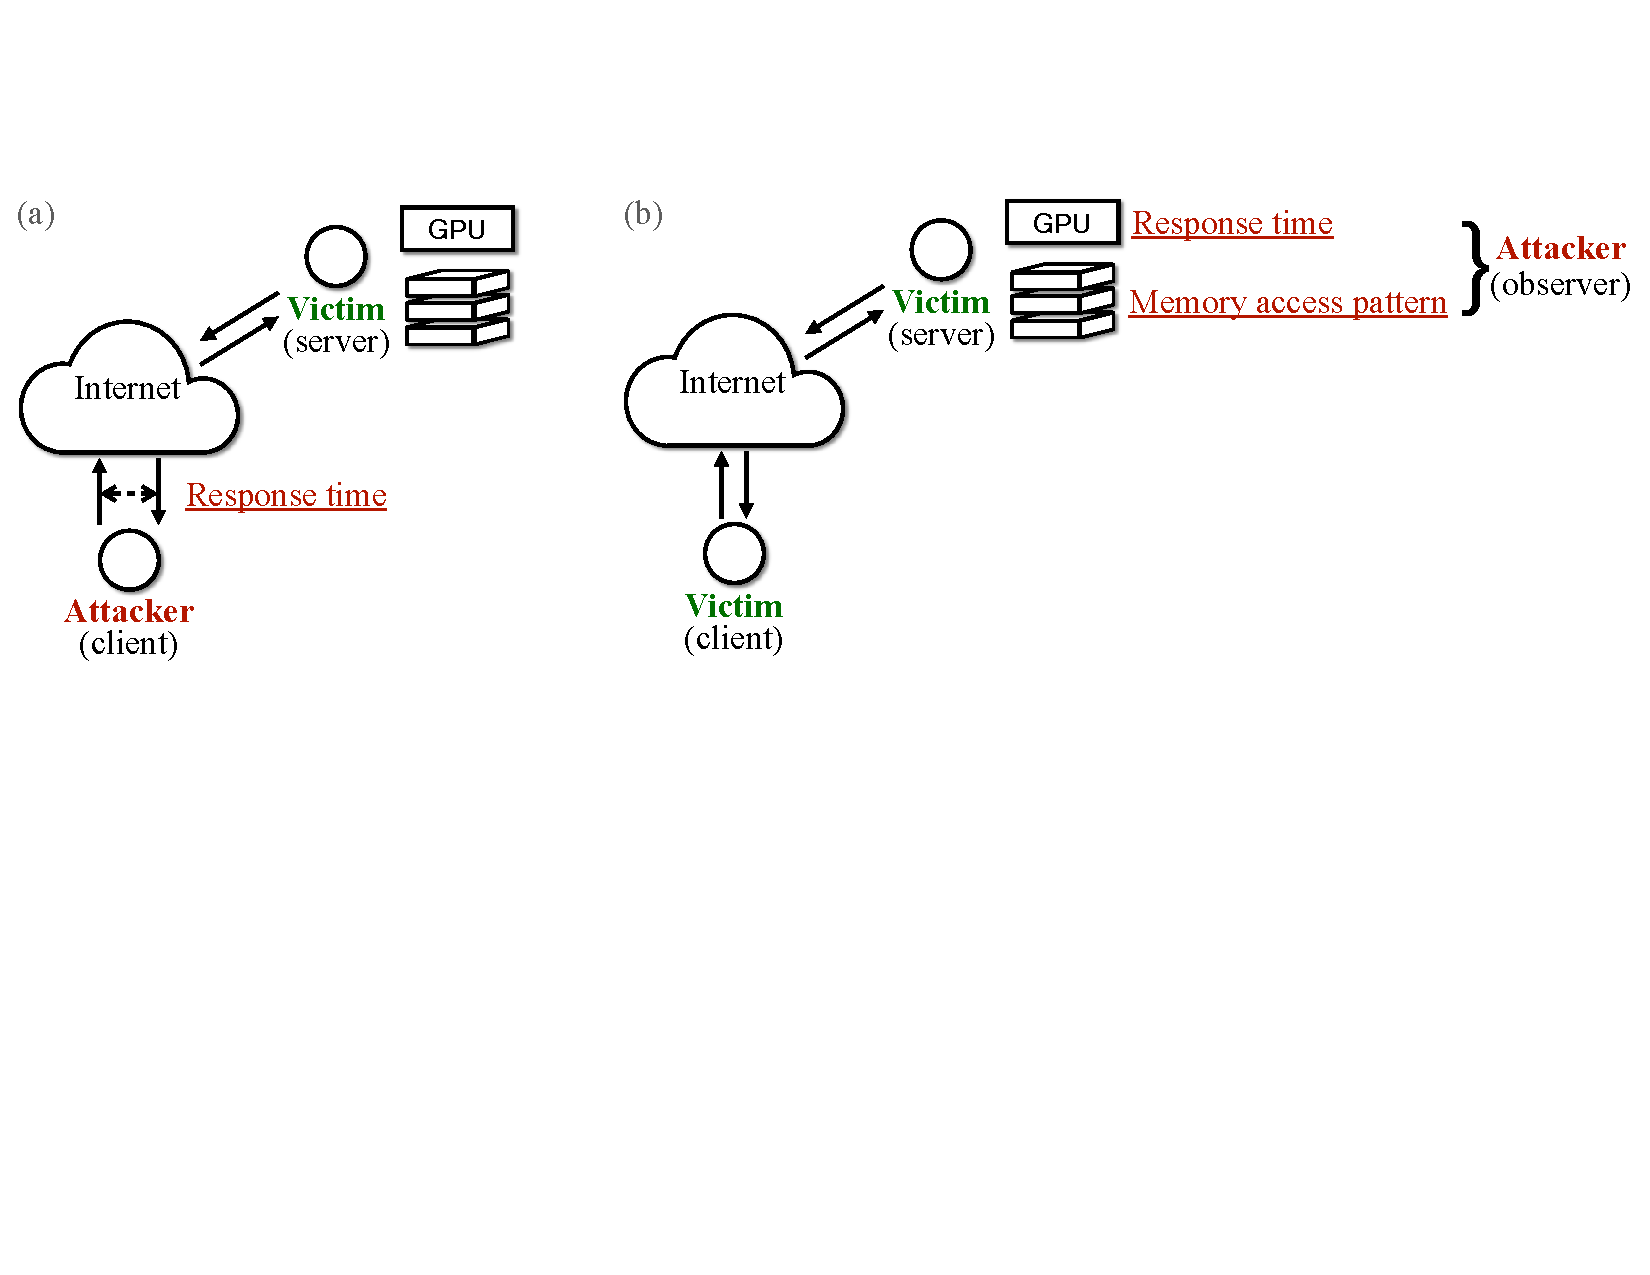
\includegraphics[clip,trim=0 10cm 0 2cm,width=0.72\pdfpagewidth]{figs/thrust1-fig.pdf}
    \caption{Attacker model considered in Thrust 1 \farzaneh{add quantitative?}}
    \label{fig:th1-attack}
    \end{figure}

\paragraph{Thrust 2. Active attacks}
The attacker has its own process in the cloud (as a client) which coexists with the victim process.
%
Te victim and attacker both use the GPU server on the cloud.
%
The attacker can gets its hand on the memory contents created by the victim process.

See Figure~\ref{fig:th2-attack}

\begin{figure}[h]
    \centering
    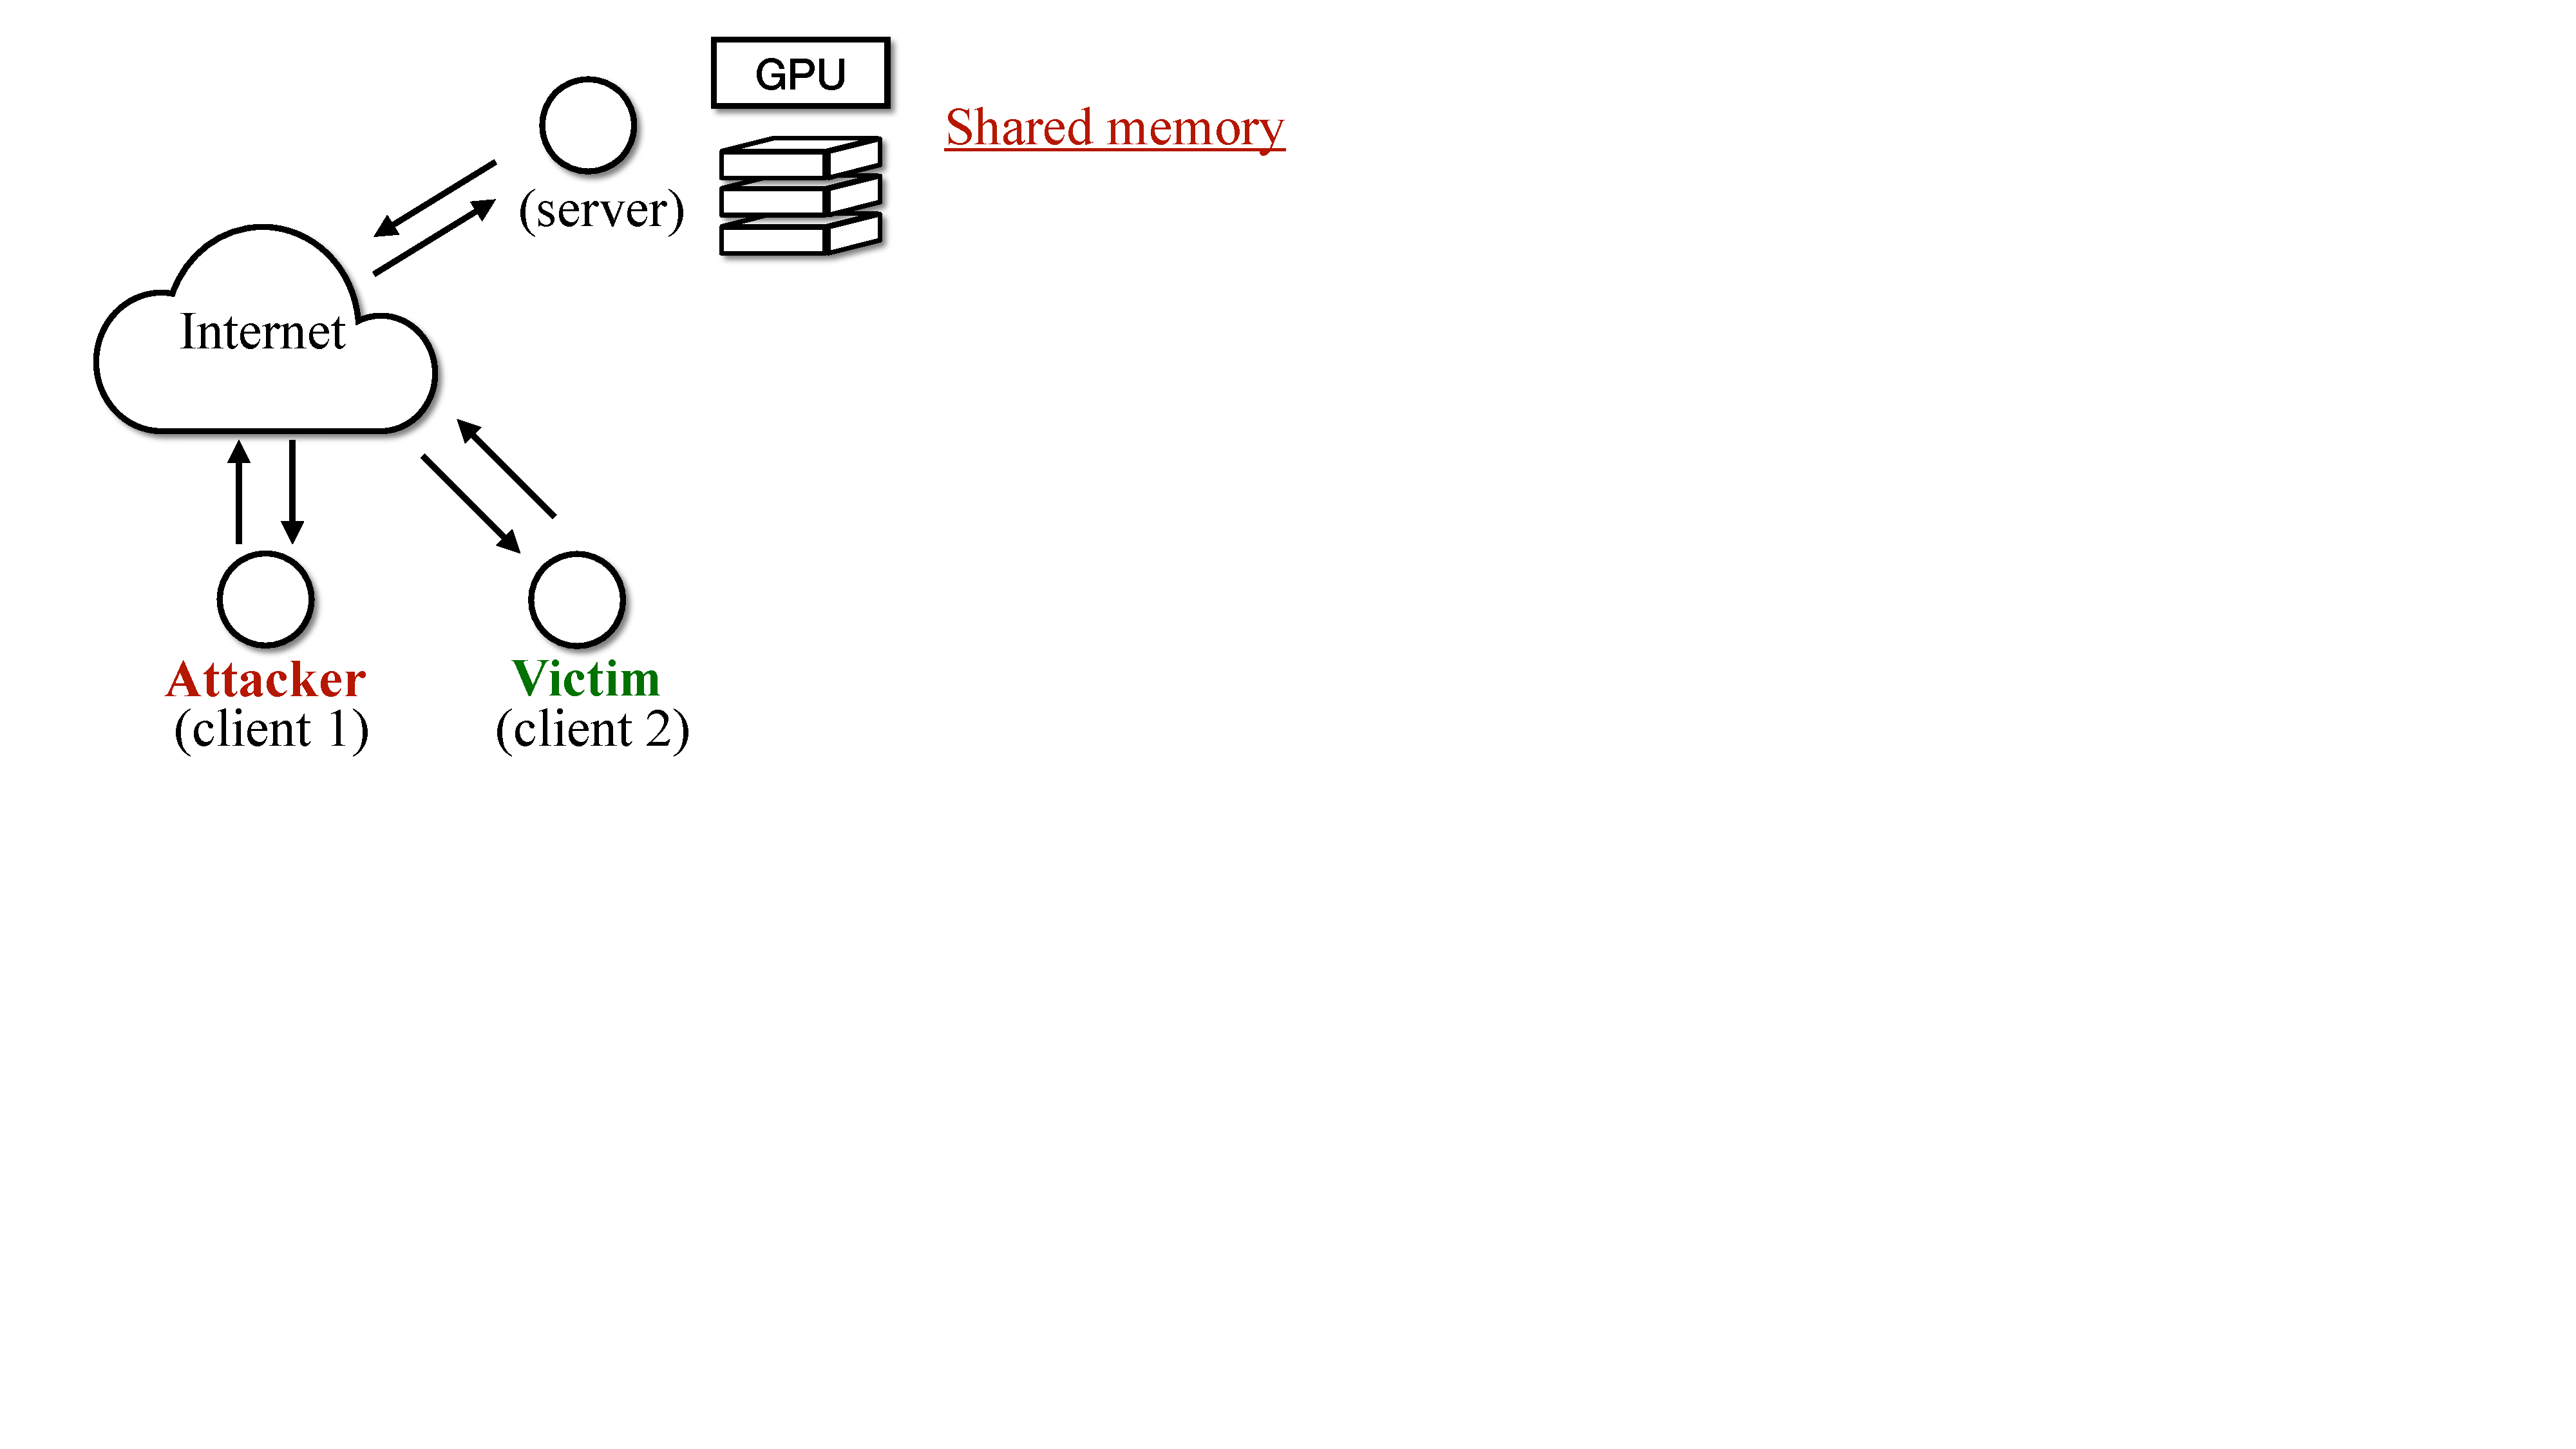
\includegraphics[clip,trim=0 17cm 10cm 0cm,width=0.72\pdfpagewidth]{figs/thrust2-fig.pdf}
    \caption{Attacker model considered in Thrust 2 \farzaneh{add more}}
    \label{fig:th2-attack}
    \end{figure}


\paragraph{Thrust 3. Case study}


In the first thrust we consider non-offensive attacks.
%
In the second thrust we consider offensive attacks.
%
We consider the unique parallelism paradigm in GPU as well as its memory behavior.

\paragraph{Related work. Type system for MiniCuda.}

\paragraph{Related works on GPU security.}
(With a microbenchmark they measured the
time for a sequence of memory accesses of each thread in a block.)
%
The attack strategy commonly deployed in CPU-based. timing attack methods consist of one block of ciphertext, and profiling the associated time to process that
block. However, on a GPU it would be the encryption workload would contain multiblock messages, and on each data sample, the GPU
timing attackwould produce many blocks of ciphertext.
The key difference is that the GPU scenario will only
collect a single timing value for the multiple blocks.
Although many successful attack methods have been
demonstrated on CPU platforms, these methods cannot be directly applied to the GPU platform due to a
lack of accurate timing information and nondeterminism in thread scheduling.

\paragraph{Symbolic GPU security.}


